\documentclass[12pt]{beamer}
\usepackage{color}
\usepackage{xcolor}
%\usepackage{latexsym}
%\usepackage{unicode-math}
\usepackage{amsmath}
\usepackage[labelfont=bf]{caption}
\usepackage{graphicx}  %package graphic
%\usepackage{siunitx}
\usepackage{tikz}
\usetikzlibrary{shapes}
\usepackage{subcaption}
%\usepackage{algorithmicx}
%\usepackage[noend]{algpseudocode}
\usetikzlibrary{automata, positioning, arrows}
\usetheme{Boadilla}   
\usepackage{xeCJK}
%\usepackage{array}
%\usepackage{tabularx}
%\usepackage{mathtools}
%\usepackage{listings}
%\usepackage{textcomp}
%\usepackage[T1]{fontenc}
%\usepackage{lmodern}
\usepackage{stmaryrd}
\usepackage{adjustbox}

\setCJKmainfont{微軟正黑體} 

\setbeamerfont{title}{size=\Large,series=\bfseries}  % title size

\setbeamerfont{frametitle}{size=\large,series=\bfseries}  % frametitle size, also can size*=<pt>

% Item include picture
\setbeamertemplate{itemize item}   % First Level item
{
\includegraphics[height=0.33cm]{../Figures/golden-earth-on-white}}

\setbeamertemplate{itemize subitem} % Second level item
{
\includegraphics[height=0.31cm]{../Figures/golden-sun-on-white}}

\setbeamertemplate{itemize subsubitem} % Third Level item
{
\includegraphics[height=0.27cm]{../Figures/golden-paw-on-white}}

\definecolor{darkgold}{rgb}{0.765 0.64 0.0} % for highlighted text in black-and-white slides

%\newtheorem{problem}{Problem}
\mode<presentation>{\newtheorem{algorithm}{Algorithm}}
\mode<article>{\newenvironment{algorithm}{}{}}
%\newtheorem{solution}{Solution}

%\renewcommand{\highlightb}{\highlightg}

%\newlength{\subtextwidth}
%\setlength{\subtextwidth}{11cm}


\title{Antichains: Alternative Algorithms for LTL Satisfiability and Model-Checking}
%\subtitle{(Based on [Manber 1989])}
\author{林宏陽}
%\institute[IM.NTU]{Department of Information Management\\ National Taiwan University}
%\date[Algorithms 2019]{\null}
\mode<presentation>{\date[SVVRL]{\null}}
\mode<article>{\date{\today}}

\begin{document}
\begin{frame}
	\maketitle
\end{frame}

\begin{frame}{Introduction}
	\begin{itemize}
		\item A model for an LTL formula over a set $P$ of propositions is an infinite word $\mathnormal{w}$ over the alphabet $\Sigma = 2^{P}$.
		\item An LTL formula $\phi$ defines a set of words $\llbracket \phi \rrbracket = \{\mathnormal{w} \in \Sigma^{\omega} \mid \mathnormal{w} \models \phi\}$.
		\item The satisfiability problem asks, given an LTL formula $\phi$, if $\llbracket \phi \rrbracket$ is empty.
		\item The model-checking problem asks, given an omega-regular language $\mathcal{L}$(e.g., the set
of all computations of a reactive system) and a LTL formula $\phi$, if $\mathcal{L} \subseteq \llbracket \phi \rrbracket$
		\item Given a LTL formula $\phi$, we can construct a NBW $\mathcal{A}_{\phi}$ such that $\text{L}_{\text{b}}(\mathcal{A}_{\phi}) = \llbracket \phi \rrbracket$
		\item This reduces the satisfiability and model-checking problems to automata-theoretic questions.
	\end{itemize}
\end{frame}

\begin{frame}{Introduction(cont'd)}
	\begin{itemize}
		\item Implemented in explicit way(such as SPIN) : worst-case exponential.
		\item Implemented in symbolic way(such as NuSMV) : it scales better.
		\item Efficient algorithms to reason on large LTL formulas are highly desirable.
		\item A new efficient way to analyze sABW (the number of states and symbolic transitions are linear in the size of the LTL formula).
		\item This approach avoids the explicit translation to NBW.
	\end{itemize}
\end{frame}

\begin{frame}{Linear Temporal Logic}
	\begin{itemize}
		\item $P$ is a finite set of propositions
		\item a Kripke structure over
$P$ is a tuple $\mathcal{K} = \langle Q, q_{\iota}, \rightarrow_{\mathcal{K}}, \mathcal{L} \rangle$
		\begin{itemize}
			\item $Q$ is a finite set of states	
			\item $q_{\iota} \in Q$ is the initial state
			\item $\rightarrow_{\mathcal{K}} \subseteq Q \times Q$ is a transition relation
			\item $\mathcal{L} : Q \to 2^{P}$ is a labeling function
		\end{itemize}
		\item A run of $\mathcal{K}$ is an infinite sequence $\rho = q_{0}q_{1}\cdots$ such that $q_{0} = q_{\iota}$ and for all $i \geq 0$, $(q_{i}, q_{i+1}) \in \rightarrow_{\mathcal{K}}$
		\item Let $\mathcal{L}(\rho) = \mathcal{L}(q_{0})\mathcal{L}(q_{1})\cdots$ and define the language of K as $\text{L}(\mathcal{K}) =
\{\mathcal{L}(\rho) \mid \rho \text{ is a run of } \mathcal{K}\}$
	\end{itemize}
\end{frame}

\begin{frame}{Linear Temporal Logic(cont'd)}
	\begin{itemize}
		\item The LTL formulas over $P$ are defined by $\phi ::= p \mid \neg\phi \mid \phi \lor \phi \mid \mathbin{\mathcal{X}}\phi \mid \phi \mathbin{\mathcal{U}} \phi$ where $p \in P$.
		\item Given an infinite word $\mathnormal{w} = \sigma_{0}\sigma_{1}\cdots \in \Sigma^{\omega}$ where $\Sigma = 2^{P}$ , and an LTL formula $\phi$ over $P$, we say that $\mathnormal{w}$ satisfies $\phi$ (written $\mathnormal{w} \models \phi$) if and only if (recursively):
		\begin{itemize}
			\item $\phi \equiv p$ and $p \in \sigma_{0}$,
			\item $\phi \equiv \neg\phi_{1}$ and $\mathnormal{w} \not\models \phi_{1}$,
			\item $\phi \equiv \phi_{1} \lor \phi_{2}$ and $\mathnormal{w} \models \phi_{1}$ or $\mathnormal{w} \models \phi_{2}$,
			\item $\phi \equiv \mathbin{\mathcal{X}}\phi_{1}$ and $\sigma_{1}\sigma_{2}\cdots \models \phi_{1}$, or
			\item $\phi \equiv \phi_{1}\mathbin{\mathcal{U}}\phi_{2}$ and for some $k \in N$, $\sigma_{k}\sigma_{k+1}\cdots \models \phi_{2}$ and for all $i$, $0 \leq i < k$,
$\sigma_{i}\sigma_{i+1}\cdots \models \phi_{1}$.
		\end{itemize}
		\item $true$, $false$ and $\phi_{1} \land \phi_{2}$ can be derived from the definition.
		\item let $\Diamond\phi = \text{true} \mathbin{\mathcal{U}}\phi$, $\Box\phi =
\neg\Diamond\neg\phi$, and $\phi_{1}\mathbin{\mathcal{R}}\phi_{2} = \neg(\neg\phi_{1}\mathbin{\mathcal{U}}\neg\phi_{2})$.
	\end{itemize}
\end{frame}

\begin{frame}{Linear Temporal Logic(cont'd)}
	\begin{itemize}
		\item The satisfiability problem : whether $\llbracket \phi \rrbracket = \emptyset$.
		
		\item The model-checking problem : whether $\mathcal{K} \models \phi$
		\begin{itemize}
			\item we say that $\mathcal{K}$ satisfies $\phi$ ($\mathcal{K} \models \phi$) if and only if $\text{L}(\mathcal{K}) \subseteq \llbracket \phi \rrbracket$
			\item that is for all runs $\rho$ of $\mathcal{K}$, we have $\mathcal{L}(\rho) \models \phi$
		\end{itemize}
		\item Both problems are PSPACE-COMPLETE.
	\end{itemize}
\end{frame}

\begin{frame}{sABW}
	\begin{itemize}
		\item Given a finite set $Q$, let $\text{Lit}(Q) = Q \cup \{\neg q \mid q \in Q\}$ be the set of literals over $Q$.
		\item $\mathcal{B}^{+}(Q)$ be the set of positive boolean formulas over $Q$ (formulas built from elements in $Q\cup\{true, false\}$ using $\land$ and $\lor$)
		\item Given $R \subseteq Q$ and $\varphi \in \mathcal{B}^{+}(Q)$, $R \models \varphi$ if and only if we assign $true$ to the
elements of $R$ and $false$ to the elements of $Q \setminus R$ satisfies $\varphi$.
	\end{itemize}
\end{frame}

\begin{frame}{sABW(cont'd)}
	\begin{itemize}
		\item A symbolic alternating Büchi automaton over the set of propositions $P$ is a tuple $\mathcal{A} = \langle \text{Loc}, I, \Sigma, \delta, \alpha \rangle$ where
		\begin{itemize}
			\item Loc is a finite set of states (or locations)
			\item $I \in \mathcal{B}^{+}(\text{Loc})$.
				\begin{itemize}
					\item A set $s \subseteq \text{Loc}$ is initial if $s \models I$.
				\end{itemize}
			\item $\Sigma = 2^{P}$ is the alphabet.
			\item $\delta : \text{Loc} \to \mathcal{B}^{+}(\text{Lit}(P)\cup\text{Loc})$ is the transition function.
			\item $\alpha \subseteq \text{Loc}$ is the set of accepting states.
		\end{itemize}
	\end{itemize}
\end{frame}


\begin{frame}{sABW(cont'd)}
	\begin{itemize}
		\item A run of $\mathcal{A}$ on an infinite word $\mathnormal{w} = \sigma_{0}\sigma_{1}\cdots \in \Sigma^{\omega}$ is a DAG $T_{\mathnormal{w}} = \langle V, V_{\iota}, \to \rangle$ where:
		\begin{itemize}
			\item $V \subseteq \text{Loc} \times N$. A node $(\ell, \mathnormal{i})$ represents the location $\ell$ after the first $\mathnormal{i}$ letters of $\mathnormal{w}$ have been read by $\mathcal{A}$. Nodes of the form $(\ell, \mathnormal{i})$ with 	$\ell \in \alpha$ are called $\alpha$-nodes;
			\item $V_{\iota} \subseteq \text{Loc} \times \{0\}$ is such that $V_{\iota} \subseteq V$ and $\{\ell \mid (\ell, 0) \in V_{\iota}\} \models I$;
			\item $\to \subseteq V \times V$ is such that for all $(\ell, \mathnormal{i}) \in V$
				\begin{itemize}
					\item if $(\ell, \mathnormal{i}) \to (\ell', \mathnormal{i}')$ then $\mathnormal{i}' = \mathnormal{i} + 1$
					\item $\sigma_{i} \cup \{\ell' \mid (\ell, \mathnormal{i}) \to (\ell', \mathnormal{i} + 1)\} \models \delta(\ell)$
				\end{itemize}
		\end{itemize}
		\item A run $T_{\mathnormal{w}}$ on an infinite word $\mathnormal{w}$ is accepting if \textcolor{red}{all} its infinite paths visit $\alpha$-nodes infinitely often.
		\item An infinite word $\mathnormal{w} \in \Sigma^{\omega}$ is accepted by $\mathcal{A}$ if there \textcolor{red}{exists} an accepting run on it.
	\end{itemize}
\end{frame}

\newcommand{\ABWExample}[1]{
\tikzset{
->, % makes the edges directed
>=stealth, % makes the arrow heads bold
every edge/.style={draw, thick, black},
node distance=0.8cm and 2.3cm, % specifies the minimum distance between two nodes. Change if necessary.
every state/.style={thick, fill=gray!10}, % sets the properties for each ’state’ node
initial text=$ $, % sets the text that appears on the start arrow
}
	\begin{figure}[ht] % ’ht’ tells LaTeX to place the figure ’here’ or at the top of the page
	\centering % centers the figure
	\begin{adjustbox}{max width=#1\textwidth, max totalheight=#1\textheight}
		\begin{tikzpicture}
			\node[draw=none] (l) {};
			\node[state, accepting, above right = 0.6cm and 1.5cm of l] (l4) {$\ell_{4}$};
			\node[state, right = of l4] (l3) {$\ell_{3}$};
			\node[state, below right =0.6cm and 1.5cm of l] (l2) {$\ell_{2}$};
			\node[state, accepting, right = of l2] (l1) {$\ell_{1}$};
			\node[draw=none, below right =0.4cm and 1cm of l3] (ll) {};
			\draw (l) edge[bend right = 25] node{} (l4);
			\draw (l) edge[bend left = 25] node{} (l2);
			\draw (l4) edge[loop above] node{$p$} (l4);
			\draw (l3) edge[loop above] node{true} (l3);
			\draw (l2) edge[loop below] node{true} (l2);
			\draw (l1) edge[loop below] node{$\neg r$} (l1);
			\draw (l4) edge node[above]{true} (l3);
			\draw (l4) edge[loop, out=0, in=-50, looseness=6] (l4);
			\draw (l2) edge node[above]{$\neg p \land \neg r$} (l1);
			\draw (l3) edge node[above]{$p$} (ll);
		\end{tikzpicture}
	\end{adjustbox}
		\caption{Alternating automaton for $\varphi \equiv \neg(\Box\Diamond p \to \Box(\neg p \to \Diamond r))$}
	\end{figure}
}


\begin{frame}{example}
	\ABWExample{0.45}
	\begin{itemize}
		\item $\ell_{4}$ and $\ell_{3}$ check that $\phi_{1} \equiv \Box\Diamond p$ holds.
		\item $\ell_{2}$ and $\ell_{1}$ check that $\phi_{2} \equiv \Diamond(\neg p \land \Box\neg r)$ holds.
		\item $\delta(\ell_{4}) = (p \land \ell_{4}) \lor (\text{true} \land \ell_{3} \land \ell_{4})$
		\item $\delta(\ell_{3}) = (\text{true}\land \ell_{3})\lor (p \land \text{true})$
	\end{itemize}
\end{frame}

\begin{frame}{sNBW}
	\begin{itemize}
		\item A nondeterministic Büchi automaton is an sABW $\mathcal{A} = \langle \text{Loc}, I, \Sigma, \delta, \alpha \rangle$ such that
		\begin{itemize}
			\item $I$ is a disjunction of locations.
			\item for all $\ell \in \text{Loc}$, $\delta(\ell)$ is a disjunction of $\varphi \land \ell'$ where $\varphi \in \mathcal{B}^{+}(\text{Lit}(P))$ and $ \ell' \in \text{Loc}$.
		\end{itemize}
		\item Define the reverse automaton of $\mathcal{A}$ as $\mathcal{A}^{-1} = \langle \text{Loc}, \alpha, \Sigma, \delta^{-1}, I \rangle$ where $\delta^{-1} = \{(\ell, \sigma, \ell') \mid (\ell', \sigma, \ell) \in \delta\}$.
	\end{itemize}
\end{frame}

\begin{frame}{Miyano-Hayashi construction}
	\begin{itemize}
		\item Transform an sABW into a sNBW.
		\item The state of sNBW is the form $\langle s, o \rangle$.
		\item $s$ is a set of states that maintains a whole level of a guessed run DAG.
		\item $o$ is a set of states that ``owe'' a visit to an accepting state.
		\item  The Büchi condition asks that $o$ gets empty infinitely often in order to ensure that \textcolor{red}{every} path of the run DAG visits accepting states infinitely often.
	\end{itemize}
\end{frame}

\begin{frame}{Miyano-Hayashi construction (cont'd)}
	
		Given an sABW $\mathcal{A} = \langle \text{Loc}, I, \Sigma, \delta, \alpha \rangle$ over $P$, let MH$(\mathcal{A}) = \langle Q, I^{\text{MH}}, \Sigma, \delta^{\text{MH}}, \alpha^{\text{MH}} \rangle$ be a sNBW where:
		\begin{itemize}
			\item $Q = 2^{\text{Loc}} \times 2^{\text{Loc}}$
			\item $I^{\text{MH}}$ is the disjunction of all the pairs $\langle s$, $\emptyset \rangle$ such that $s \models I$
		
		\item $\delta^{\text{MH}}$ is defined for all $\langle s, o \rangle \in Q$:
		\begin{itemize}
			\item if $o \neq \emptyset$, then $\delta^{\text{MH}}(\langle s, o \rangle)$ is the disjunction of all the formulas $\varphi \land \langle s', o' \setminus \alpha \rangle$ with $\varphi \in \mathcal{B}^{+}(\text{Lit}(P))$ such that
			\begin{itemize}
				\item $o' \subseteq s'$
				\item $\forall \ell \in s \cdot \forall \sigma \subseteq P$ : if $\sigma \models \varphi$ then $\sigma \cup s' \models \delta(\ell)$
				\item $\forall \ell \in o \cdot \forall \sigma \subseteq P$ : if $\sigma \models \varphi$ then $\sigma \cup o' \models \delta(\ell)$
			\end{itemize}
			
			\item if $o = \emptyset$, then $\delta^{\text{MH}}(\langle s, o \rangle)$ is the disjunction of all the formulas $\varphi \land \langle s', s' \setminus \alpha \rangle$ with $\varphi \in \mathcal{B}^{+}(\text{Lit}(P))$ such that
			\begin{itemize}
				\item $\forall \ell \in s \cdot \forall \sigma \subseteq P$ : if $\sigma \models \varphi$ then $\sigma \cup s' \models \delta(\ell)$
			\end{itemize}
		\end{itemize}
		\item $\alpha^{\text{MH}} = 2^{\text{Loc}} \times \{\emptyset\}$
		\end{itemize}
	\begin{theorem}
		For all sABW $\mathcal{A}$, we have $\text{L}_{\text{b}}(\text{MH}(\mathcal{A})) = \text{L}_{\text{b}}(\mathcal{A})$.
	\end{theorem}
\end{frame}

\begin{frame}{Recall ABW}
	\ABWExample{1}
\end{frame}

\begin{frame}{After Miyano-Hayashi construction}
\tikzset{
%->, % makes the edges directed
>=stealth, % makes the arrow heads bold
every edge/.style={draw, thick, black},
node distance=0.8cm and 2.3cm, % specifies the minimum distance between two nodes. Change if necessary.
every state/.style={thick, fill=gray!10}, % sets the properties for each ’state’ node
initial text=$ $, % sets the text that appears on the start arrow
}
	\begin{figure}[t] % ’ht’ tells LaTeX to place the figure ’here’ or at the top of the page
	\centering % centers the figure
	\begin{adjustbox}{max width=.95\textwidth, max totalheight=.95\textheight}
		\begin{tikzpicture}
			\node[state] (a) {$\langle \{\ell_{2}, \ell_{4}\}, \{\ell_{2}\}\rangle$};
			\node[state, initial, accepting, left = of a] (1) {$\langle \{\ell_{2}, \ell_{4}\}, \emptyset$};
			\node[state, above right = and 4.5cm of a] (b) {$\langle \{\ell_{2}, \ell_{3},\ell_{4}\}, \{\ell_{2}\}\rangle$};
			\node[state, above left = of b] (2) {$\langle \{\ell_{2}, \ell_{3}, \ell_{4}\}, \{\ell_{2}, \ell_{3}\}\rangle$};
			\node[state, above right = of b] (3) {$\langle \{\ell_{2}, \ell_{3}, \ell_{4}\}, \{\ell_{3}\}\rangle$};
			\node[state, accepting, below right = of a] (c) {$\langle \{\ell_{1}, \ell_{3},\ell_{4}\}, \emptyset\rangle$};
			\node[state, accepting, right = of c] (d) {$\langle \{\ell_{1}, \ell_{4}\}, \emptyset\rangle$};
			\node[state, right = of d] (e) {$\langle \{\ell_{1}, \ell_{3},\ell_{4}\}, \{\ell_{3}\}\rangle$};


			\draw (3.north west) edge[->, bend right = 100] node[left]{$\{p\}, \{p, r\}$} (1);
			\draw (1) edge[->] node[above]{$\{p\}, \{p, r\}$} (a);
			\draw (1) edge[->, bend left = 20] node[above]{$\emptyset, \{p\}, \{r\}, \{p, r\}$} (2);
			\draw (1) edge[->, bend right = 40] node[below]{$\emptyset$} (e);
			\draw (2) edge[loop right] node{$\emptyset, \{p\}, \{r\}, \{p, r\}$} (2);
			\draw (2.south) edge[->, bend right = 15] node[above]{$\{p\}, \{p, r\}$} (b);
			\draw (2.north east) edge[->, bend left = 10] node[above]{$\emptyset$} (3);
			\draw (3) edge[loop above] node{$\emptyset, \{p\}, \{r\}, \{p, r\}$} (3);
			\draw (3) edge[->, bend left = 20] node[right]{$\emptyset$} (e);
			\draw (a) edge[loop above] node{$\{p\}, \{p, r\}$} (a);
			\draw (a) edge[->, bend left = 15] node[above = 0.5cm]{$\emptyset, \{p\}, \{r\}, \{p, r\}$} (b);
			\draw (b) edge[->, bend left = 15] node[below = 0.3cm]{$\{p\}, \{p, r\}$} (a);
			\draw (b) edge[loop right] node{$\emptyset, \{p\}, \{r\}, \{p, r\}$} (b);
			\draw (b) edge[->] node[right]{$\emptyset$} (c);
			\draw (a) edge[->] node[above]{$\emptyset$} (c);
			\draw (c) edge[loop left] node{$\emptyset, \{p\}$} (c);
			\draw (c) edge[->] node[below]{$\{p\}$} (d);
			\draw (d) edge[loop above] node{$\{p\}$} (d);
			\draw (d) edge[->, bend left = 15] node[above]{$\emptyset, \{p\}$} (e);
			\draw (e) edge[->, bend left = 15] node[below]{$\{p\}$} (d);
			\draw (e) edge[loop right] node{$\emptyset, \{p\}$} (e);
		\end{tikzpicture}
	\end{adjustbox}
		%\caption{After the Miyano-Hayashi construction}
	\end{figure}
\end{frame}

\begin{frame}{Satisfiability-Checking of LTL}
	\begin{itemize}
		\item Recall : The satisfiability problem for LTL asks, given an LTL formula $\phi$, if $\llbracket \phi \rrbracket$ is empty.
	\item Equivalent to check the emptiness of $\text{MH}(\mathcal{A}_{\phi})$.
	\item $\llbracket \phi \rrbracket = \text{L}_\text{b}(\mathcal{A}_{\phi}) = \emptyset$ iff $I^{\text{MH}}\cap\mathcal{F}_{\phi} = \emptyset$ where $\mathcal{F}_{\phi}$ is
	$$\mathcal{F}_{\phi} \equiv \nu y \cdot \mu x \cdot (\text{Pre}(x) \cup (\text{Pre}(y) \cap \alpha^{\text{MH}})) $$
	where $\text{Pre}(L) = \{q \in Q \mid \exists \sigma \in \Sigma \cdot \exists q' \in L : \sigma \cup \{q'\} \models \delta^{\text{MH}}(q)\}$.
	\item We call $\mathcal{F}_{\phi}$ a \textcolor{red}{backward} algorithm.
	\end{itemize}
\end{frame}

\begin{frame}{Satisfiability-Checking of LTL(cont'd)}
	\begin{itemize}
		\item The following fixpoint formulas compute the accepting reachable states $R_{\alpha}$ and then the set $\mathcal{F}'_{\phi}$ in a \textcolor{red}{forward} fashion.

		$$R_{\alpha} \equiv \alpha^{\text{MH}} \cap \mu x \cdot (\text{Post}(x) \cup I^{\text{MH}})$$
		$$\mathcal{F}'_{\phi} \equiv \nu y \cdot \mu x \cdot (\text{Post}(x) \cup (\text{Post}(y) \cap R_{\alpha})) $$
		
		where $\text{Post}(L) = \{q \in Q \mid \exists \sigma \in \Sigma \cdot \exists q' \in L : \sigma \cup \{q\} \models \delta^{\text{MH}}(q')\}$.
	\end{itemize}
	\begin{theorem}
		$\text{L}_{\text{b}}(\mathcal{A}_{\phi}) = \emptyset ~ iff ~ \mathcal{F}'_{\phi} = \emptyset$.
	\end{theorem}
\end{frame}

\begin{frame}{Proof}
	\begin{itemize}
		\item Define $\Delta^{\text{MH}} : Q \times \Sigma^{+}$ the extension of the transition relation $\delta^{\text{MH}}$(recursively)
		\begin{itemize}
			\item $\Delta^{\text{MH}}(q, \sigma) = \delta^{\text{MH}}(q, \sigma)$
			\item $\Delta^{\text{MH}}(q, \mathnormal{w}\sigma) = \{q' \in Q \mid \exists q'' \in \Delta^{\text{MH}}(q, \mathnormal{w}) : \sigma \cup \{q'\} \models \delta^{\text{MH}}(q'')\}$ for each $q \in Q$, $\mathnormal{w} \in \Sigma^{+}$ and $\sigma \in \Sigma$.
		\end{itemize}
		\item Looping states $\mathcal{C}^{\text{MH}} = \{q \in Q \mid \exists \mathnormal{w} \in \Sigma^{+} : q \in \Delta^{\text{MH}}(q,\mathnormal{w})\}$
		\item From the definition of Büchi acceptance condition for NBW, we have $\text{L}_{\text{b}}(\mathcal{A}_{\phi}) = \emptyset$ iff $\mathcal{C}^{\text{MH}} \cap R_{\alpha} = \emptyset$.
	\end{itemize}
\end{frame}

\begin{frame}{Proof(cont'd)}
	\begin{itemize}
		\item Let $\text{HM}(\mathcal{A}_{\phi})$ be the reverse automaton.
		\item The following equivalences establish the theorem:
		\begin{itemize}
				\item $\nu y \cdot \mu x \cdot (\text{Pre}(x) \cup (\text{Pre}(y) \cap R_{\alpha})) = \emptyset$
				\item iff $\mathcal{C}^{\text{MH}} \cap R_{\alpha} = \emptyset$
				\item iff $\mathcal{C}^{\text{HM}} \cap R_{\alpha} = \emptyset$
				\item iff $\nu y \cdot \mu x \cdot (\text{Post}(x) \cup (\text{Post}(y) \cap R_{\alpha})) = \emptyset$
				\item iff $\mathcal{F}'_{\phi} = \emptyset$
		\end{itemize}
	\end{itemize}
\end{frame}

\begin{frame}{Closed Sets and Antichains}
	\begin{itemize}
		\item Let $\preceq \subseteq Q \times Q$ be a preorder.
		\item $q_{1} \prec q_{2}$ iff $q_{1} \preceq q_{2}$ and $q_{2} \npreceq q_{1}$
		\item A set $R \subseteq Q$ is \textcolor{red}{$\preceq$-closed} iff for all $q_{1}, q_{2} \in Q$, if $q_{1} \preceq q_{2}$ and $q_{2} \in R$ then $q_{1} \in R$.
		\item The \textcolor{red}{$\preceq$-closure} of $R$, is the set $\llbracket R \rrbracket_{\preceq} = \{q \in Q \mid \exists q' \in R : q \preceq q'\}$.
		\item Let $\lceil R \rceil_{\preceq} = \{q \in R \mid \nexists q' \in R : q \prec q'\}$ be the set of \textcolor{red}{$\preceq$-maximal elements} of $R$.
		\item Let $\lfloor R \rfloor_{\succeq} = \{q \in R \mid \nexists q' \in R : q \succ q'\}$ be the set of \textcolor{red}{$\succeq$-minimal elements} of $R$.
		\item For all $\preceq$-closed sets $R \subseteq Q$, $R = \llbracket \lceil R \rceil_{\preceq} \rrbracket_{\preceq}$.
		\item For all $\succeq$-closed sets $R \subseteq Q$, $R = \llbracket \lfloor R \rfloor_{\succeq} \rrbracket_{\succeq}$.
		\item if $\preceq$ is a partial order, then $\lceil R \rceil_{\preceq}$ is an \textcolor{red}{antichain}.
	\end{itemize}
\end{frame}

\begin{frame}{Simulation}
	\begin{itemize}
		\item Let $\mathcal{A} = \langle \text{Loc}, I, \Sigma, \delta, \alpha \rangle$ be an NBW.
		\item A preorder $\preceq \subseteq \text{Loc} \times \text{Loc}$ is a \textcolor{red}{forward-simulation} for $\mathcal{A}$ if for all $q_{1}, q_{2}, q_{3} \in \text{Loc}$, for all $\sigma \in \Sigma$,
		\begin{itemize}
			\item if $q_{1} \preceq q_{2}$ and $q_{2} \xrightarrow{\sigma}_{\delta} q_{3}$ then there exists $q_{4} \in \text{Loc}$ such that $q_{1} \xrightarrow{\sigma}_{\delta} q_{4}$ and $q_{4} \preceq q_{3}$, and
			\item if $q_{1} \preceq q_{2}$ and $q_{2} \in \alpha$ then $q_{1} \in \alpha$.
		\end{itemize}
	\end{itemize}

\tikzset{
%->, % makes the edges directed
>=stealth, % makes the arrow heads bold
every edge/.style={draw, thick, black},
node distance=0.8cm and 2.3cm, % specifies the minimum distance between two nodes. Change if necessary.
every state/.style={thick, fill=gray!10}, % sets the properties for each ’state’ node
initial text=$ $, % sets the text that appears on the start arrow
}
	\begin{figure}[ht] % ’ht’ tells LaTeX to place the figure ’here’ or at the top of the page
	\centering % centers the figure
	\begin{adjustbox}{max width=0.9\textwidth, max totalheight=\textheight}
		\begin{tikzpicture}
			\node[] (then) {then};
			\node[state, above left = of then] (l2) {$q_{3}$};
			\node[state, left = of l2] (l1) {$q_{2}$};
			\node[below = of l1] (mid) {
			\begin{tikzpicture}
      		\node [rotate=90] {$\preceq$};    
    		\end{tikzpicture}
};
			\node[state, below = of mid] (l3) {$q_{1}$};
			\node[below left = of l1] (if) {If};
			
			\node[state, below right = of then] (l3') {$q_{1}$};
			\node[state, right = of l3'] (l4') {$q_{4}$};
			\node[above = of l4'] (mid') {
			\begin{tikzpicture}
      		\node [rotate=90] {$\preceq$};    
    		\end{tikzpicture}
};
			\node[state, above = of mid'] (l2') {$q_{3}$};
			
			\node[above = of l3'] (mid'') {
			\begin{tikzpicture}
      		\node [rotate=90] {$\preceq$};    
    		\end{tikzpicture}
};
			\node[state, above = of mid''] (q2') {$q_{2}$};

			\draw (l1) edge[->] node[above] {$\sigma$} (l2);
			\draw (l3') edge[->] node[above] {$\sigma$} (l4');
			\draw (q2') edge[->] node[above] {$\sigma$} (l2');
			
			\draw (l1) edge[dashed] (mid);
			\draw (mid) edge[dashed] (l3);
			\draw (l4') edge[dashed] (mid');
			\draw (mid') edge[dashed] (l2');
			\draw (mid'') edge[dashed] (l3');
			\draw (mid'') edge[dashed] (q2');
			
		\end{tikzpicture}
	\end{adjustbox}
		\caption{Forward-simulation}
	\end{figure}
\end{frame}

\begin{frame}{Simulation}
	\begin{itemize}
		\item A \textcolor{red}{backward-simulation} for $\mathcal{A}$ is a forward-simulation for $\mathcal{A}^{-1}$.
		\item Recall $\mathcal{A}^{-1} = \langle \text{Loc}, \alpha, \Sigma, \delta^{-1}, I \rangle$ where $\delta^{-1} = \{(\ell, \sigma, \ell') \mid (\ell', \sigma, \ell) \in \delta\}$.
		\item A preorder $\succeq \subseteq \text{Loc} \times \text{Loc}$ is a \textcolor{red}{backward-simulation} for $\mathcal{A}$ if for all $q_{1}, q_{2}, q_{3} \in \text{Loc}$, for all $\sigma \in \Sigma$,
		\begin{itemize}
			\item if $q_{1} \succeq q_{2}$ and $q_{3} \xrightarrow{\sigma}_{\delta} q_{2}$ then there exists $q_{4} \in \text{Loc}$ such that $q_{4} \xrightarrow{\sigma}_{\delta} q_{1}$ and $q_{4} \succeq q_{3}$, and
			\item if $q_{1} \succeq q_{2}$ and $q_{2} \in I$ then $q_{1} \in I$.
		\end{itemize}
	\end{itemize}

\tikzset{
%->, % makes the edges directed
>=stealth, % makes the arrow heads bold
every edge/.style={draw, thick, black},
node distance=0.8cm and 2.3cm, % specifies the minimum distance between two nodes. Change if necessary.
every state/.style={thick, fill=gray!10}, % sets the properties for each ’state’ node
initial text=$ $, % sets the text that appears on the start arrow
}
	\begin{figure}[ht] % ’ht’ tells LaTeX to place the figure ’here’ or at the top of the page
	\centering % centers the figure
	\begin{adjustbox}{max width=0.9\textwidth, max totalheight=\textheight}
		\begin{tikzpicture}
			\node[] (then) {then};
			\node[state, above left = of then] (l2) {$q_{1}$};
			\node[below = of l2] (mid) {
			\begin{tikzpicture}
      		\node [rotate=90] {$\preceq$};    
    		\end{tikzpicture}
};
			\node[state, below = of mid] (l3) {$q_{2}$};
			\node[state, left = of l3] (l1) {$q_{3}$};
			\node[above left = 1.5cm and 1cm of l1] (if) {If};
			
			\node[state, below right = of then] (l3') {$q_{3}$};
			\node[state, right = of l3'] (l4') {$q_{2}$};
			\node[above = of l4'] (mid') {
			\begin{tikzpicture}
      		\node [rotate=90] {$\preceq$};    
    		\end{tikzpicture}
};
			\node[state, above = of mid'] (l2') {$q_{1}$};
			
			\node[above = of l3'] (mid'') {
			\begin{tikzpicture}
      		\node [rotate=90] {$\preceq$};    
    		\end{tikzpicture}
};
			\node[state, above = of mid''] (q2') {$q_{4}$};

			\draw (l1) edge[->] node[above] {$\sigma$} (l3);
			\draw (l3') edge[->] node[above] {$\sigma$} (l4');
			\draw (q2') edge[->] node[above] {$\sigma$} (l2');
			
			\draw (l2) edge[dashed] (mid);
			\draw (mid) edge[dashed] (l3);
			\draw (l4') edge[dashed] (mid');
			\draw (mid') edge[dashed] (l2');
			\draw (mid'') edge[dashed] (l3');
			\draw (mid'') edge[dashed] (q2');
			
		\end{tikzpicture}
	\end{adjustbox}
		\caption{Backward-simulation}
	\end{figure}
\end{frame}

\begin{frame}{Simulation(cont'd)}
	\begin{itemize}
		\item A \textcolor{red}{backward-simulation} for $\mathcal{A}$ is a forward-simulation for $\mathcal{A}^{-1}$.
		\item It is not true in general that $\succeq$ is a backward-simulation for $\mathcal{A}$ if $\preceq$ is a forward-simulation for $\mathcal{A}$.
		\item It is not true in general that $\preceq$ is a forward-simulation for $\mathcal{A}^{-1}$ if $\preceq$ is a forward-simulation for $\mathcal{A}$.
		\item It is not true in general that $\succeq$ is a backward-simulation for $\mathcal{A}$ if $\succeq$ is a backward-simulation for $\mathcal{A}^{-1}$.
		\item Consider a state $q_{c}$ that has no predecessor and such that $q_{b} \preceq q_{c}$
	\end{itemize}
\end{frame}

\begin{frame}{Simulation(cont'd)}
	\tikzset{
		%->, % makes the edges directed
		every cross out node/.append style={-,solid},
		>=stealth, % makes the arrow heads bold
		every edge/.style={draw, thick, black},
		node distance=0.8cm and 2.3cm, % specifies the minimum distance between two nodes. Change if necessary.
		every state/.style={thick, fill=gray!10}, % sets the properties for each ’state’ node
		initial text=$ $, % sets the text that appears on the start arrow
		}
	\begin{figure}
	\begin{subfigure}{.4\linewidth}
		\centering % centers the figure
		\begin{adjustbox}{max width=0.9\textwidth, max totalheight=\textheight}
		\begin{tikzpicture}
			\node[] (mid') {
			\begin{tikzpicture}
			  \node [rotate=90] {$\preceq$}; 
			\end{tikzpicture}
	};
			\node[state, above = 0.5cm of mid'] (qc) {$q_{c}$};
			\node[state, below = 0.5cm of mid'] (qb) {$q_{b}$};
			\node[state, left = 3cm of qb] (qa) {$q_{a}$};
			\node[draw = none, left = 3cm of qc] (qd) {};
			
			\draw (qc) edge[dashed] node {} (mid');
			\draw (qb) edge[dashed] node {} (mid');
			\draw (qa) edge[->] node[above] {$\sigma$} (qb);
			\draw (qd) edge[->] node[draw=red, cross out] {} (qc);
		\end{tikzpicture}
		\end{adjustbox}
		\subcaption*{$\mathcal{A}$}
	\end{subfigure}
		\begin{subfigure}{.4\linewidth}
			\centering % centers the figure
			\begin{adjustbox}{max width=0.9\textwidth, max totalheight=\textheight}
			\begin{tikzpicture}
				\node[] (mid') {
				\begin{tikzpicture}
				  \node [rotate=90] {$\succeq$}; 
				\end{tikzpicture}
		};
				\node[state, above = 0.5cm of mid'] (qc) {$q_{c}$};
				\node[state, below = 0.5cm of mid'] (qb) {$q_{b}$};
				\node[state, left = 3cm of qb] (qa) {$q_{a}$};
				\node[draw = none, left = 3cm of qc] (qd) {};
				
				\draw (qb) edge[dashed] node {} (mid');
				\draw (qc) edge[dashed] node {} (mid');
				\draw (qb) edge[->] node[above] {$\sigma$} (qa);
				\draw (qc) edge[->] node[draw=red, cross out] {} (qd);
			\end{tikzpicture}
			\end{adjustbox}
		\subcaption*{$\mathcal{A}^{-1}$}
		\end{subfigure}
	\end{figure}

	\begin{itemize}
		\item Suppose $\succeq$ is a backward-simulation for an sNBW $\mathcal{A}$. By definition of backward-simulation, $q_{c} \succeq q_{b}$ in $\mathcal{A}$ implies $q_{c} \preceq q_{b}$ in $\mathcal{A}^{-1}$.
		\item However, $q_{c}$ has no successor in $\mathcal{A}^{-1}$, contradict with the definition of forward-simulation . 
	\end{itemize}
\end{frame}

\begin{frame}{Simulation(cont'd)}
	\label{lemma}
	\begin{itemize}
		\item The following lemma shows that the language of a sNBW is unchanged if we add a transition from a state $q_{a}$ to $q_{c}$ which is forward-simulated by one of the successors of $q_{a}$.
		\item By adding in this way all the possible transitions, we
		obtain a sNBW for which $\succeq$ is a backward-simulation.
	\end{itemize}
	\begin{lemma}
		Let $\mathcal{A}$ be an sNBW with transition relation $\delta_{\mathcal{A}}$ and $\preceq$ be a forward-simulation relation for $\mathcal{A}$. If $(q_{a}, \sigma, q_{b}) \in \delta_{\mathcal{A}}$ and $q_{b} \preceq q_{c}$, then the sNBW $\mathcal{A}'$ that differs from $\mathcal{A}$ only by its transition relation $\delta_{\mathcal{A}'} = \mathcal{A} \cup \{(q_{a}, \sigma, q_{c})\}$ defines the same language as $\mathcal{A}$, that is $\text{L}_\text{b}(\mathcal{A}') = \text{L}_\text{b}(\mathcal{A})$.
	\end{lemma}
\end{frame}


\begin{frame}{Simulation(cont'd)}
	\tikzset{
		%->, % makes the edges directed
		>=stealth, % makes the arrow heads bold
		every edge/.style={draw, thick, black},
		node distance=0.8cm and 2.3cm, % specifies the minimum distance between two nodes. Change if necessary.
		every state/.style={thick, fill=gray!10}, % sets the properties for each ’state’ node
		initial text=$ $, % sets the text that appears on the start arrow
		}
	\begin{figure}[ht] % ’ht’ tells LaTeX to place the figure ’here’ or at the top of the page
		\centering % centers the figure
			\begin{tikzpicture}
				\node[] (mid') {
				\begin{tikzpicture}
				  \node [rotate=90] {$\preceq$}; 
				\end{tikzpicture}
	};
				\node[state, above = 0.5cm of mid'] (qc) {$q_{c}$};
				\node[state, below = 0.5cm of mid'] (qb) {$q_{b}$};
				\node[state, left = 3cm of qb] (qa) {$q_{a}$};
	
				\draw (qa) edge[->] node[above] {$\sigma$} (qb);
				\draw (qb) edge[dashed] node {} (mid');
				\draw (qc) edge[dashed] node {} (mid');
				\only<2>{
					\draw (qa) edge[->, red] node[above] {$\sigma$} (qc);
				}
			\end{tikzpicture}
			\caption{Lemma on slide~\pageref{lemma}}
		\end{figure}
		\only<1>{
			\begin{itemize}
				\item $(q_{a}, \sigma, q_{b}) \in \delta_{\mathcal{A}}$ and $q_{b} \preceq q_{c}$
			\end{itemize}
		}
		\only<2>{
			\begin{itemize}
				\item The new sNBW preserves the same language.
				\item Furthermore, $\succeq$ is a backward-simulation now.
			\end{itemize}
		}
\end{frame}

\begin{frame}{Simulation(cont'd)}
	\begin{itemize}
		\item Given a backward-simulation $\succeq$ for $\text{MH}(\mathcal{A}_{\phi})$, all the sets that are computed to evaluate $\mathcal{R}_{\alpha}$ and $\mathcal{F}'_{\phi}$ are $\succeq$-closed, that is $I^{\text{MH}}$ and $\alpha^{\text{MH}}$ are $\succeq$-closed, and $x \cap y$, $x \cup y$ and $\text{\textcolor{red}{Post}}(x)$ are $\succeq$-closed whenever $x$ and $y$ are $\succeq$-closed.
		\item Recall
		
		$$\mathcal{R}_{\alpha} \equiv \alpha^{\text{MH}} \cap \mu x \cdot (\text{Post}(x) \cup I^{\text{MH}})$$
		$$\mathcal{F}'_{\phi} \equiv \nu y \cdot \mu x \cdot (\text{Post}(x) \cup (\text{Post}(y) \cap \mathcal{R}_{\alpha})) $$
	\end{itemize}
\end{frame}

\begin{frame}{Simulation(cont'd)}
	\tikzset{
		%->, % makes the edges directed
		every cross out node/.append style={-,solid},
		>=stealth, % makes the arrow heads bold
		every edge/.style={draw, thick, black},
		node distance=0.8cm and 2.3cm, % specifies the minimum distance between two nodes. Change if necessary.
		every state/.style={thick, fill=gray!10}, % sets the properties for each ’state’ node
		initial text=$ $, % sets the text that appears on the start arrow
		}
	\begin{figure}[ht]
		\centering
		\begin{tikzpicture}
			\draw[thick] (2.5,0) parabola (2.5+1.5,4) ;
			\draw[thick] (2.5,0) parabola (2.5-1.5,4) ;

			\draw[thick] (-2.5,0) parabola (-2.5+1.5,4) ;
			\draw[thick] (-2.5,0) parabola (-2.5-1.5,4) ;

			\node (Postx) at (2.5, 5) {Post($\mathnormal{x}$)} ;
			\node (x) at (-2.5, 5) {$\mathnormal{x}$} ;

			\node[state] (q1) at (2.5, 1.5) {$\mathnormal{q}_{1}$};
			\node[] (mid) at (2.5, 2.5) {
				\begin{tikzpicture}
				  \node [rotate=90] {$\preceq$}; 
				\end{tikzpicture}
			};
			\node[state] (q2) at (2.5, 3.5) {$\mathnormal{q}_{2}$};
			\node[state] (q3) at (-2.5, 1.5) {$\mathnormal{q}_{3}$};

			\draw (q3) edge[->] node[above] {$\sigma$} (q1);

			\only<2>{
				\node[state, fill=red!10] (q4) at (-2.5, 3.5) {$\textcolor{red}{\mathnormal{q}_{4}}$};
				\node[] (mid) at (-2.5, 2.5) {
					\begin{tikzpicture}
				  		\node [rotate=90] {$\textcolor{red}{\preceq}$}; 
					\end{tikzpicture}
				};

				\draw (q4) edge[->, red] node[above] {$\textcolor{red}{\sigma}$} (q2);
			}
		  \end{tikzpicture}
		  \caption{$\text{Post}(\mathnormal{x})$ is $\succeq$-closed whenever $\mathnormal{x}$ is $\succeq$-closed.}
	\end{figure}
	
\end{frame}

\begin{frame}{Simulation(cont'd)}
	\begin{itemize}
		\item The relation $\preceq_{\text{alt}}$ defined by $\langle s, o \rangle \preceq_{\text{alt}} \langle s', o' \rangle$ iff
		\begin{itemize}
			\item $s \subseteq s'$
			\item $o \subseteq o'$
			\item $o = \emptyset$ iff $o' = \emptyset$
		\end{itemize}
		is a forward-simulation for $\text{MH}(\mathcal{A}_{\phi})$.
		\item According to the Lemma on slide~\pageref{lemma}, the relation $\succeq_{\text{alt}}$ (which is $\preceq_{\text{alt}}^{-1}$) is a backward-simulation if we modify the transition relation of $\text{MH}(\mathcal{A}_{\phi})$ as follows : if $\delta^{\text{MH}}(\langle s, o \rangle)$ is a disjunction of formulas of the form $\varphi \land \langle s', o' \rangle$ with $\varphi \in \mathcal{B}^{+}(\text{Lit}(P))$, then we disjunctively add all the formulas $\varphi \land \langle s'', o'' \rangle$ to $\delta^{\text{MH}}(\langle s, o \rangle)$ such that $\langle s', o' \rangle \preceq_{\text{alt}} \langle s'', o'' \rangle$.
		\item We keep only the $\succeq_{\text{alt}}$-minimal elements of $\succeq_{\text{alt}}$-closed sets to evaluate $\mathcal{F}'_{\phi}$.
		\begin{itemize}
			\item The intuition is that if there is no accepting run from $\langle s, o \rangle$ then there is no accepting run from any pair $\langle s', o' \rangle \succeq_{\text{alt}} \langle s, o \rangle$.
		\end{itemize}
	\end{itemize}
\end{frame}

\begin{frame}{Simulation(cont'd)}
	\tikzset{
		%->, % makes the edges directed
		>=stealth, % makes the arrow heads bold
		every edge/.style={draw, thick, black},
		node distance=0.8cm and 2.3cm, % specifies the minimum distance between two nodes. Change if necessary.
		every state/.style={thick, fill=gray!10}, % sets the properties for each ’state’ node
		initial text=$ $, % sets the text that appears on the start arrow
		}
	\begin{figure}[ht] % ’ht’ tells LaTeX to place the figure ’here’ or at the top of the page
		\centering % centers the figure
			\begin{tikzpicture}
				\node[] (mid') {
				\begin{tikzpicture}
				  \node [rotate=90] {$\preceq_{\text{alt}}$}; 
				\end{tikzpicture}
	};
				\node[state, above = 0.5cm of mid'] (qc) {$\langle \textnormal{s}'', \textnormal{o}'' \rangle$};
				\node[state, below = 0.5cm of mid'] (qb) {$\langle \textnormal{s}', \textnormal{o}' \rangle$};
				\node[state, left = 3cm of qb] (qa) {$\langle \textnormal{s}, \textnormal{o} \rangle$};
	
				\draw (qa) edge[->] node[above] {$\sigma \models \varphi$} (qb);
				\draw (qb) edge[dashed] node {} (mid');
				\draw (qc) edge[dashed] node {} (mid');
				\only<2>{
					\draw (qa) edge[->, red] node[above left] {$\sigma \models \varphi$} (qc);
				}
			\end{tikzpicture}
		\end{figure}
		\only<1>{
			\begin{itemize}
				\item $\delta^{\text{MH}}(\langle s, o \rangle) = \varphi \land \langle s', o' \rangle$ and $\langle s', o' \rangle \preceq_{\text{alt}} \langle s'', o'' \rangle$
			\end{itemize}
		}
		\only<2>{
			\begin{itemize}
				\item $\delta^{\text{MH}}(\langle s, o \rangle) = (\varphi \land \langle s', o' \rangle) \textcolor{red}{\lor (\varphi \land \langle s'', o'' \rangle)}$, the new sNBW preserves the same language.
				\item Furthermore, $\succeq_{\text{alt}}$ is a backward-simulation now.
			\end{itemize}
		}
\end{frame}

\begin{frame}{Elements of efficient implementation}
	\begin{itemize}
		\item Combine BDDs and antichains to compute the $\succeq_{\text{alt}}$-minimal elements of $\text{Post}(\llbracket \cdot \rrbracket_{\succeq_{\text{alt}}})$ efficiently.
		\item Antichains of pairs $\langle s, o \rangle$ are represented \textit{explicitly} (as a list of pairs of sets
		of locations) while computation of the successors of a pair $\langle s, o \rangle$ is done \textit{symbolically}.
		\item Given a BDD $B$ over a set of variables $V$ (seen as a boolean formula over $V$), let $\llbracket B \rrbracket$ be the set of truth assignments over $V$ that satisfy $B$.
		\item Given a pair $\langle s, o \rangle$, Algorithm 1 computes the set $L_{\text{Post}} = \lfloor \text{Post}(\llbracket \{\langle s, o \rangle\}\rrbracket_{\succeq_{\text{alt}}})\rfloor_{\succeq_{\text{alt}}}$.
	\end{itemize}
\end{frame}

\begin{frame}{Semi-symbolic Algorithm for Post($\cdot$)}
	\label{Algorithm1_part1}
	\begin{center}
		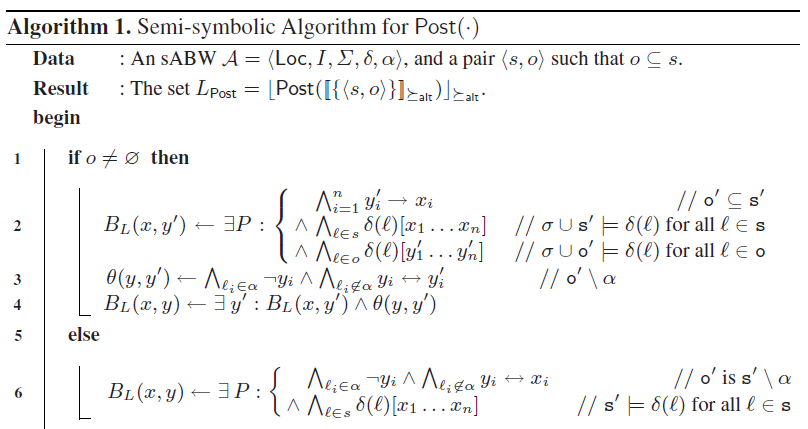
\includegraphics[scale=0.5]{Algorithm1_part1}
	\end{center}
	\begin{minipage}{.5\textwidth}
		\begin{itemize}
			\item The algorithm uses the intermediate boolean variables to encode respectively the sets 
		\end{itemize}
	\end{minipage}%
	\begin{minipage}{.5\textwidth}
		\small
		\centering
		\begin{tabular}{ ||c|c|| } 
			\hline
			boolean variables & set \\
			\hline \hline
			$\mathnormal{x}_{1},\dots , \mathnormal{x}_\mathnormal{n}$ & $s'$ \\
			\hline 
			$\mathnormal{y}_{1},\dots , \mathnormal{y}_\mathnormal{n}$ & $o' \setminus \alpha$ \\ 
			\hline
			$\mathnormal{y}~'_{1},\dots , \mathnormal{y}~'_\mathnormal{n}$ & $o'$ \\ 
			\hline
		\end{tabular}
	\end{minipage}
\end{frame}

\begin{frame}{Semi-symbolic Algorithm for Post($\cdot$)}
	\label{Algorithm1_part2}
	\begin{center}
		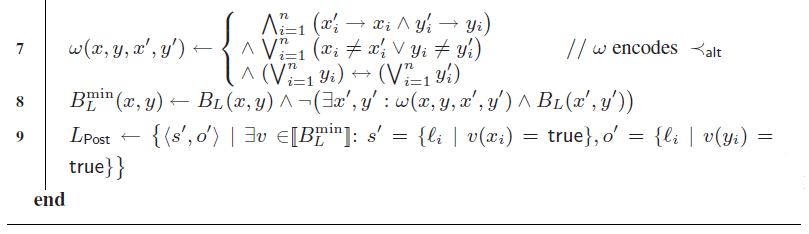
\includegraphics[scale=0.5]{Algorithm1_part2}
	\end{center}
	\begin{minipage}{.5\textwidth}
		\begin{itemize}
			\item Using a BDD $\omega (\mathnormal{x}, \mathnormal{y}, \mathnormal{x}', \mathnormal{y}')$ that encodes the relation $\prec_{\text{alt}}$ (we have $\langle s', o' \rangle \prec_{\text{alt}} \langle s, o \rangle$ in $\omega$ where $s, o, s', o'$ encoded respectively as the table) 
		\end{itemize}
	\end{minipage}%
	\begin{minipage}{.5\textwidth}
		\small
		\centering
		\begin{tabular}{ ||c|c|| } 
			\hline
			boolean variables & set \\
			\hline \hline
			$\mathnormal{x}$ & $s$ \\
			\hline 
			$\mathnormal{y}$ & $o$ \\
			\hline
			$\mathnormal{x}~'$ & $s'$ \\
			\hline
			$\mathnormal{y}~'$ & $o'$ \\ 
			\hline
		\end{tabular}
	\end{minipage}
\end{frame}

\begin{frame}{Semi-symbolic Algorithm for $\text{Post}(\cdot)$}
	\begin{itemize}
		% \item When computing the successors of a pair $\langle s, o \rangle$, the algorithm uses the intermediate boolean variables to encode respectively the sets 
		% 	\begin{center}
		% 		\begin{tabular}{ ||c|c|| } 
		% 			\hline
		% 			boolean variables & set \\
		% 			\hline \hline
		% 			$\mathnormal{x}_{1},\dots , \mathnormal{x}_\mathnormal{n}$ & $s'$ \\
		% 			\hline 
		% 			$\mathnormal{y}_{1},\dots , \mathnormal{y}_\mathnormal{n}$ & $o' \setminus \alpha$ \\ 
		% 			\hline
		% 			$\mathnormal{y}~'_{1},\dots , \mathnormal{y}~'_\mathnormal{n}$ & $o'$ \\ 
		% 			\hline
		% 		\end{tabular}
		% 	\end{center}
		% where $\langle s', o' \setminus \alpha \rangle \in \text{Post}(\llbracket \{ \langle s, o \rangle \} \rrbracket_{\succeq_{\text{alt}}})$.
	
		\item $\delta(\ell)[\mathnormal{x}_{1} \cdots \mathnormal{x}_\mathnormal{n}]$ denotes the formula
		$\delta(\ell)$ in which each occurrence of a location $\ell_{\mathnormal{i}}$ is replaced by variable $\mathnormal{x}_{\mathnormal{i}}$ for all $1 \leq \mathnormal{i} \leq \mathnormal{n}$.
		\item The existential quantification over the set $P$ of propositions ($\exists P$) matches
		the definition of the $\text{Post}(\cdot)$ operator.
		\item Recall $\text{Post}(L) = \{q \in Q \mid \exists \sigma \in \Sigma \cdot \exists q' \in L : \sigma \cup \{q\} \models \delta^{\text{MH}}(q')\}$.
	\end{itemize}
\end{frame}

\begin{frame}{LTL Model-Checking}
	\begin{itemize}
		\item Given a Kripke structure $\mathcal{K} = \langle Q, q_{\iota}, \rightarrow_{\mathcal{K}}, \mathcal{L} \rangle$ and and an LTL formula $\phi$, the model-checking problem for $\mathcal{K}$ and $\phi$ reduces to the emptiness of $\text{L}(\mathcal{K}) \cap \text{L}_\text{b}(\mathcal{A}_{\neg \phi})$ (where $\mathcal{A}_{\neg \phi} = \langle \text{Loc}, I, \Sigma, \delta, \alpha \rangle$ is the sABW for $\neg \phi$) which can be checked by computing the following fixpoint formulas over the lattice of subsets of $Q \times 2^{\text{Loc}} \times 2^{\text{Loc}}$ :
		
		$$\mathcal{R}_{\alpha}^{\mathcal{K}} \equiv \alpha' \cap \mu \mathnormal{x} \cdot (\text{Post}_{\text{MC}}(\mathnormal{x}) \cup I~')$$
		$$\mathcal{F}_{\phi}^{\mathcal{K}} \equiv \nu \mathnormal{y} \cdot \mu \mathnormal{x} \cdot (\text{Post}_{\text{MC}}(\mathnormal{x}) \cup (\text{Post}_{\text{MC}}(\mathnormal{y}) \cap \mathcal{R}_{\alpha}^{\mathcal{K}}))$$

		\begin{itemize}
			\item $\text{Post}_{\text{MC}}(L) = \{(q', \langle s', o' \rangle) \mid \exists (q, \langle s, o \rangle) \in L : q \rightarrow_{\mathcal{K}} q' \land \mathcal{L}(q) \cup \{\langle s', o' \rangle\} \models \delta^{\text{MH}}(\langle s, o \rangle)\}$
			\item $I~' = \{q_{\iota}\} \times I^{\text{MH}}$
			\item $\alpha' = Q \times \alpha^{\text{MH}}$
		\end{itemize}
		\item $\mathcal{F}_{\phi}^{\mathcal{K}} = \emptyset$ iff $\text{L}(\mathcal{K}) \cap \text{L}_{\text{b}}(\mathcal{A}_{\neg \phi}) = \emptyset$ iff $\mathcal{K} \models \phi$.
	\end{itemize}
\end{frame}

\begin{frame}{LTL Model-Checking (cont'd)}
	\begin{itemize}
		\item There exists a partial order $\succeq_{\text{MC}}$ for which all the sets that are computed to evaluate $\mathcal{F}_{\phi}^{\mathcal{K}}$ are $\succeq_{\text{MC}}$-closed.
		\item The relation $\succeq_{\text{MC}}$ is defined by $(q, \langle s, o \rangle) \succeq_{\text{MC}} (q', \langle s', o' \rangle)$ iff $q = q'$ and $\langle s, o \rangle \succeq_{\text{alt}} \langle s', o' \rangle$.
	\end{itemize}
\end{frame}

\begin{frame}{LTL Model-Checking (cont'd)}
	\begin{itemize}
		\item Use a semi-symbolic forward algorithm for model-checking.
		\item Assume
		a symbolic representation of $\mathcal{K}$ where each state $q \in Q$ is a valuation for a finite set
		of boolean variables $V = \{\mathnormal{z}_{1}, \cdots , \mathnormal{z}_{\mathnormal{m}}\}$ such that $P \subseteq V$.
		\item The labeling function $\mathcal{L}$ is defined as the projection of $2^{V}$ to $2^{P}$ in the natural way.
		\item The transition relation is given
		by a BDD $T(V, V~')$ over $V \cup V~'$ where the set $V~' = \{\mathnormal{z}' \mid \mathnormal{z} \in V\}$ of primed variables
		is used to define the value of the variables after the transition.
	\end{itemize}
\end{frame}

\begin{frame}{LTL Model-Checking (cont'd)}
	\begin{itemize}
		\item To efficiently compute $\mathcal{F}_{\phi}^{\mathcal{K}}$, we need a compact representation of $succeq_{\text{MC}}$-antichains. Consider a semisymbolic representation of antichains, as a set of pairs $(B, \langle s, o \rangle)$ where $B$ is a BDD over $V$.
		\begin{itemize}
			\item A pair $(B, \langle s, o \rangle)$ represents the set $\llbracket (B, \langle s, o \rangle) \rrbracket = \{(q, \langle s, o \rangle) \mid q \in \llbracket B \rrbracket\}$.
		\end{itemize}
		\item Let $L = \{(q_{1}, \langle s_{1},  o_{1} \rangle), (q_{2}, \langle s_{2}, o_{2} \rangle), \cdots \}$ be an $\succeq_{\text{MC}}$-antichain.
		\item Let $S_{L} = \{\langle s, o \rangle \mid \exists (q, \langle s, p \rangle) \in L\}$.
		\item Define $R(L) = \{(B, \langle s, o \rangle) \mid \langle s, o \rangle \in S_{L} \land \llbracket B \rrbracket = \{q \mid (q, \langle s, o \rangle) \in L \} \}$.
	\end{itemize}
	\begin{lemma}
		If $L$ is an $\succeq_{\text{MC}}$-antichain for all $(B_{1}, \langle s_{1}, o_{1} \rangle), (B_{2}, \langle s_{2}, o_{2} \rangle) \in R(L)$, if $\langle s_{1}, o_{1} \rangle \succ_{\text{alt}} \langle s_{2}, o_{2} \rangle$, then $\llbracket B_{1} \rrbracket \cap \llbracket B_{2} \rrbracket = \emptyset$.
	\end{lemma}
\end{frame}

\begin{frame}{LTL Model-Checking (cont'd)}
	\begin{itemize}
		\item We say that $R(L)$ is a \textit{semi-symbolic} and \textit{canonical} representation of $\llbracket L \rrbracket_{\succeq_{\text{MC}}}$.
		\item The algorithm
		to compute $\text{Post}_{\text{MC}}(\cdot)$ follows the lines of Algorithm 1 on slide~\pageref{Algorithm1_part1} and~\pageref{Algorithm1_part2}, using $2n$ boolean variables
		to encode a pair $\langle s, o \rangle$.
		\item The existential quantification over $V$ is performed after synchronization over propositions $P$ with the Kripke structure.
		\item Let $B_{L}(\mathnormal{x}, \mathnormal{y}, V)$ be the
		BDD that encodes with variables $\mathnormal{x}, \mathnormal{y}$ the successors of $\langle s, o \rangle$ over a symbolic label encoded by variables $V$.
		\item We compute the BDD $C_{L}(\mathnormal{x}, \mathnormal{y}, V~') = \exists V : B(V) \land T(V, V~') \land B_{L}(\mathnormal{x}, \mathnormal{y}, V)$ and then we construct the encoding $R(\cdot)$ of its minimal elements.
	\end{itemize}
\end{frame}

\end{document}